\documentclass[a4paper,11pt]{article}

\usepackage{amsmath,amssymb,amsfonts,amsthm}    % Typical maths resource packages
\usepackage{graphicx}                           % Packages to allow inclusion of graphics
\usepackage{hyperref}                           % For creating hyperlinks in cross references
\usepackage[authoryear]{natbib}                 % literature reference style
\usepackage[bf]{caption2}
%for table
\usepackage{adjustbox}
\usepackage{graphicx} 
\usepackage[flushleft]{threeparttable}

% For code listing
\usepackage{listings}
\lstset{language=R, 	basicstyle=\footnotesize,numbers=left,stepnumber=1,	showstringspaces=false,tabsize=1,breaklines=true,	breakatwhitespace=false,
}

%\renewcommand\thesection{\Roman{section}}
%\renewcommand\thesubsection{\Alph{subsection}}



% -------------------------------
% --- some layout definitions ---
% -------------------------------

% define topline
\usepackage[automark]{scrpage2}
\pagestyle{scrheadings}
\automark{section}
\clearscrheadings
\ohead{\headmark}

% define citation style
\bibliographystyle{ecta}

% define page size, margin size
\setlength{\headheight}{1.1\baselineskip}
\voffset=-2cm
\hoffset=-3cm
\textheight24cm
\textwidth15.5cm
\topmargin1cm
\oddsidemargin3cm
\evensidemargin3cm

% define line line spacing = 1.5
\renewcommand{\baselinestretch}{1.5}

% define second level for `itemizing'
\renewcommand{\labelitemii}{-}




% --------------------------------------
% --------------------------------------
% --------------------------------------
% --- the structure the tex document ---
% ---  (this our recommendation) -------
% frontmatter:
%   - titlepage (mandatory),
%   - acknowledgement,
%   - abstract,
%   - table of contents (mandatory),
%   - list of abbreviations (not mandatory),
%   - list of figures (not mandatory),
%   - list of tables  (not mandatory) .
%
% body of the thesis (the structure of the thesis body is not mandatory, but the list of literature is mandatory):
%   - introduction,
%   - methods,
%   - data,
%   - results,
%   - conclusion,
%   - literature (mandatory),
%   - appendix (figures, tables).
%
% last page:
%   - declaration of authorship (mandatory).
% --------------------------------------
% --------------------------------------
% --------------------------------------

\begin{document}

% -------------------------------
% --- frontmatter: Title page ---
% -------------------------------

\thispagestyle{empty}
\begin{center}

    {\Large{\bf Income and Democracy}} \vspace{0.5cm}


    {\normalsize Bachelor's/Master's Thesis submitted\\\vspace{0.5cm}
    to}\\\vspace{0.5cm}
    {\normalsize{\bf Prof. Dr. Nikolaus Hautsch}} \\\vspace{0.5cm}
    {\normalsize Humboldt-Universit\"at zu Berlin \\
    School of Business and Economics \\
    Institute for Statistics and Econometrics \\
    Chair of Econometrics} \vspace{1cm}


    {\normalsize by \\\vspace{0.5cm}
    {\bf your name} \\
    (your matriculation number)} \vspace{1cm}


    {\normalsize in partial fulfillment of the requirements \\
    for the degree of \\
    {\bf Bachelor/Master of Science} \\
    Berlin, September 30, 2007}

\end{center}




% ------------------------------------
% --- frontmatter: Acknowledgement ---
% ------------------------------------
%\newpage
%\pagestyle{plain}
%\pagenumbering{roman}   % define page number in roman style
%\setcounter{page}{1}    % start page numbering
%\section*{Acknowledgement}

I would like to thank




% -----------------------------
% --- frontmatter: Abstract ---
% -----------------------------
\newpage
\section*{Abstract}

This is the template for a thesis at the Chair of Econometrics of
Humboldt--Universit\"at zu Berlin. A popular approach to write a
thesis or a paper is the IMRAD method (Introduction, Methods,
Results and Discussion). This approach is not mandatory! You can
find more information about formal requirements in the booklet
`Hinweise zur Gestaltung der \"au\ss eren Form von Diplomarbeiten'
which is available in the office of studies.\\

The abstract should not be longer than a paragraph of around 10 to
15 lines (or about 150 words). The abstract should contain a
concise description of the econometric/economic problem you
analyse and of your results. This allows the busy reader to obtain
quickly a clear idea of the thesis content.




% -----------------------------
% --- frontmatter: Contents ---
% -----------------------------
\newpage
\tableofcontents
\clearpage



% ----------------------------------------------------
% --- frontmatter: List of Figures (not mandatory) ---
% ----------------------------------------------------
\newpage
\addcontentsline{toc}{section}{List of Abbreviations}
\ohead[]{LIST OF ABBREVIATIONS}
\section*{List of Abbreviations}

\begin{tabular}{rp{0.2cm}lp{1cm}rp{0.2cm}l}

%%Table 2  
F\_pols     & &  Fixed Pooled OLS && && \\
fhpolriigaug    & & Augmented Freedom House Political Rights Index && &&  \\
lrgdpch  & &  Log real GDP per capita (PWT)  &&  && \\ 
sample   & & Dummy for base sample && &&\\
code&& Country code    && &&   \\
year &&    Year of observation   && &&    \\     
country    & & Country name    && &&     \\
F\_fols & &  Fixed effect OLS   && &&     \\
F\_folswod    & & Fixed effect without lagged democracy   && &&   \\
O\_fols     & &  Anual data fixed effect OLS    && &&    \\ 
T\_fols   & & Ten-year data fixed effect OLS  && &&     \\
Tw\_fols     & &      Twenty-year data fixed Effect OLS    && &&       \\
%% Table 3        
Pooled\_pols\_p    & &   Pooled OLS with PolityI\hspace{-.1em}V index   && &&    \\
polity4    & & PolityI\hspace{-.1em}V index  && &&    \\
FE\_fols\_p\_2     & &       Fixed OLS with PolityI\hspace{-.1em}V index   && &&   \\
FE\_folswod\_p     & &  Fixed OLS with PolityI\hspace{-.1em}V index without lagged democracy   && &&   \\
EF\_fols\_p\_6    & & Annua data fixed OLS with PolityI\hspace{-.1em}V index    && &&   \\
FE\_fols\_p\_7     && Ten-year data fixed OLS with PolityI\hspace{-.1em}V index  && &&   \\  
FE\_fols\_p\_9    & &   Twenty-year data fixed OLS with PolityI\hspace{-.1em}V index   && &&    \\
F\_fols\_b& &  Balance panel data fixed effect OLS       && &&     \\
%% Table 4    
samplebalancefe && Dummy for alanced sample for fixed effects   && &&   \\
F\_fols\_c    & & Base sample data without former socialist countries fixed effect OLS   && &&    \\
socialist& &   Dummy for Soviet Block, including iron curtain    && &&    \\
lpop & &  Log(total population in thousands)   && &&   \\
medage& &  Median age in population      && &&    \\
age\_veryyoung    & & Percent population age 0-15   && &&   \\
age\_young& &    Percent population age 15-30    && &&   \\
age\_midage    & & Percent population age 30-45   && &&    \\
age\_old& &    Percent population age 45-60      && &&     \\
F\_fols\_add   & &  Base sample fixed effect OLS  && &&   \\      
F\_fols\_we& &      Base sample fixed effect OLS without education   && &&    \\  
%%  Table 5
TwoSLS\_4  && Fixed effects 2SLS with lagged log GDP per capita  && &&   \\
F\_pols\_inst  && Pooled cross section OLS &&  &&  \\
F\_folswod\_inst  &&  Fixed effects OLS without lagged democracy && &&    \\
TwoSLS\_1  &&  Fixed effects 2SLS with lagged democracy and lagged log GDP per capita   && &&   \\
nsave  && Nominal savings rate: (Y-C-G)/Y  &&  &&  \\
Firststage\_4  &&  First stage regression with (t-2) lagged savings rate  && &&   \\
TwoSLS\_5  &&  Fixed effects 2SLS with lagged democracy and lagged log GDP per capita && &&   \\
Firststage\_5  &&  First stage regression with lagged democracy and (t-2) lagged savings rate && &&    \\
TwoSLS\_7  &&  Fixed effects 2SLS with lagged log GDP per capita and  lagged labor share && &&   \\
laborshare  && \% labor share of gross value added  &&   &&  \\
Firststage\_7  && First stage regression with lagged labor share and (t-2) lagged savings rate  && &&    \\
TwoSLS\_8  &&  Fixed effects 2SLS with (t-2) and (t-3) lagged democracy  && &&   \\   
Firststage\_8  &&  First stage regression with (t-2) and (t-3) lagged democracy and (t-2) lagged savings rate  && &&   \\       
%%  Figures
ave1990s & & Data set of average of Freedom House index and log GDP per capita in 1990s  && &&   \\
change\_FH& &     Data set of change of Freedom House measure of democracy and GDP per capita   && &&   \\
change\_polity4  & & Data set of change of PolityI\hspace{-.1em}V index and GDP per capita  && &&   \\
X5yr\_panel &&  Data set of five-year interval   && &&   \\

\end{tabular}




% ----------------------------------------------------
% --- frontmatter: List of Figures (not mandatory) ---
% ----------------------------------------------------
\newpage
\addcontentsline{toc}{section}{List of Figures}
\ohead[]{\rightmark}
\listoffigures


\begin{itemize}
\item F1
\end{itemize}
\\
\begin{lstlisting}
library(maptools)

pointLabel(x=F1_revise$lrgdpch,y=F1_revise$fhpolrigaug,labels=F1_revise$code,col="black")
\end{lstlisting}
\\
\\

We handle around 150 data in a figure and if we just plot by "text" command, we cannot distinguish each label. Therefore, we introduce "maptools" package for the figure in order to fix place of each label automatically to be able to recognize each one. "pointLabel" is a command to function automatically adjustment of "maptools" package. We need same texts to call "pointLabel" command with "text" command which uses to change labels form dots to specific names. 
\\
\\

\begin{itemize}
 \item F5
\end{itemize}
\\
\\

\begin{lstlisting}
x<-1945
for (i in 1:11) {
  x<-x+5
  plot(fhpolrigaug~lrgdpch,data=X5yr_panel, subset=year==x,
       xlim=c(6,10),ylim=c(0,1),ann=F, xaxt="n",yaxt="n")  #setting for length of graph by xlim and ylim, and erase whole title and axis by ann=F
  text(6.3,0.95,x, cex=1.5)              #label setting for each graph
  if (i %in% c (8:11) ) { axis (1 , col = " black ", col.axis= " black ", at = seq (6 , 10 , 2) ) }
  if (i %in% c(1 , 5 , 9) ) { axis (2 , col = " black ", col.axis = " black ", at = seq (0 , 1 , 0.5) ) }
  result<-lm(formula=fhpolrigaug~lrgdpch, data=X5yr_panel, subset=year==x)
  abline(result, col="blue")
  box(col = "grey60")
}
\end{lstlisting}

\\

\\

Figure5 shows each year panel data in each separate graph. Since we should make 11 figures and avoid to use same command for 11 times, we use "for" command to iterate same command for 11 times. We introduce a variable "x" in the command to refer each year data.  Variable "x" is added 5 for each repeat and through this, the command can refer same number of year data with "x" from data set. Also, we add "if" command to add tick mark to 1st, 5th, and 9th graph in vertical axis and 8th to 11th in horizontal axis. Through this command, "axis" command function in typical number of variable "i" which means number of iterate.


% ---------------------------------------------------
% --- frontmatter: List of Tables (not mandatory) ---
% ---------------------------------------------------
\newpage
\addcontentsline{toc}{section}{List of Tables}
\listoftables
\begin{table}[hbtp]
  \caption{Descriptive Statistics}
  \label{table:data_type}
  \small
  \centering
  \begin{tabular}{cccc}
    \hline
      & All countries  &  High-income\ countries & Low-income\ countries \\
    \hline \hline
    Panel A  &   &  & \\
    Freedom House measure of   & 0.57   & 0.78 & 0.36\\
    democracy & (0.36) & (0.30) & (0.30) \\
    Log GDP per capita_{t-1} \\(chain  weighted  1996  price)  & 8.16  & 9.02 & 7.30 \\
    Observations  &  945  &  473 & 472 \\
    Countries  &  150  &  93 & 98 \\
    \hline
    Panel B &  & & \\
    Polity measure of democracy_t & 0.57 & 0.79 &0.36 \\
      & (0.38) & (0.31) & (0.31) \\
    Observation & 854 & 427 & 427 \\
    Countries & 136 & 81 & 88 \\
    \hline
  
  \end{tabular}
\end{table}\\
Note: Panel A refers to the sample in Table ??; Panel B refers to the sample in Table ??. 


% -------------------------------
% --- main body of the thesis ---
% -------------------------------
\newpage
\pagestyle{plain}
\setcounter{page}{1}    % start page numbering anew
\pagenumbering{arabic}  % page numbers in arabic style


\section{Introduction: Sharon, Soichi}

\begin{itemize}

    \item What is the subject of the study? Describe the
        economic/econometric problem.

    \item What is the purpose of the study (working hypothesis)?

    \item What do we already know about the subject (literature
        review)? Use citations: {\it \citet{Gallant:87} shows that...
        Alternative Forms of the Wald test are considered
        \citep{Breusch&Schmidt:88}.}

    \item What is the innovation of the study?

    \item Provide an overview of your results.


    \item Outline of the paper:\\
        {\it The paper is organized as follows. The next section describes the
        model under investigation. Section \ref{Sec:Data} describes the data set
        and Section \ref{Sec:Results} presents the results. Finally, Section
        \ref{Sec:Conc} concludes.}

    \item The introduction should not be longer than 4 pages.

\end{itemize}

\section{Statistical Theory: Hyerin}\label{Sec:Theory and Design}
Describe the statistical theory that you implement and the corresponding algorithm(s) that was (were) designed. Avoid describing how the design was produced, rather, show different versions of the design if relevant.
\begin{itemize}
\item Panel Data analysis
\item Fixed Effects
\item Clustering by group
\item Instrumental Variable
\end{itemize}

\newpage
\section{Implementation}\label{Sec:Implementation}

Show the implementation. The goal of this section is to show and explain the most important parts of the code. Listing the code with highlighting and possibly line numbering is essential.
Explain the code by referring to line numbers, function calls and variable names.
Leave out trivial parts (initialization, parameter-tuning, etc...).
\begin{itemize}
	\item PLM
	\item CLSE
	\item Stargazer
	\item Figure
	
	\begin{itemize}
		\item F1
	\end{itemize}
	\\
	\begin{lstlisting}
	library(maptools)
	
	result=lm(fhpolrigaug~lrgdpch,data=ave1990s)
	R2=signif(summary(result)$r.squared,digit=4)
	R="R^2="
	
	plot(fhpolrigaug~lrgdpch,data=ave1990s,col="white",
	ylab="Freedom House measure of democracy",xlab="Log GDP per pacita(Penn World Tables)",
	sub=paste(R,R2))
	pointLabel(x=ave1990s$lrgdpch,y=ave1990s$fhpolrigaug,labels=ave1990s$code,col="black")
	
	abline(result)
	\end{lstlisting}
	\\
	\\
	
	In the paper, we insert figures to visualize the relationship between income and democracy. To
	generate Figure 2, due to the fact that we are analyzing a panel dataset which involves around
	150 country data, we cannot simply plot the data by the ”text” command because we cannot
	distinguish each label in that way. Therefore, we introduce the ”maptools” package in order
	to fix the location of each label automatically for them to be distinguishable. ”pointLabel” is
	a command to function automatically adjustment of ”maptools” package. When we replace
	pointLabel with text in line 10, we will be able to change the labels from dots to specific
	country names.
	\\
	\\
	
	\begin{itemize}
		\item F5
	\end{itemize}
	\\
	\\
	
	\begin{lstlisting}
x=1945
for (i in 1:11) {
x=x+5
plot(fhpolrigaug~lrgdpch,data=X5yr_panel, subset=year==x,
xlim=c(6,10),ylim=c(0,1),ann=F, xaxt="n",yaxt="n")  #setting for length of graph by xlim and ylim, and erase whole title and axis by ann=F
text(6.3,0.95,x, cex=1.5)     #label setting for each graph
if (i %in% c (8:11) ) { axis (1 , col = " black ", col.axis= " black ", at = seq (6 , 10 , 2) ) }
if (i %in% c(1 , 5 , 9) ) { axis (2 , col = " black ", col.axis = " black ", at = seq (0 , 1 , 0.5) ) }
result<-lm(formula=fhpolrigaug~lrgdpch, data=X5yr_panel, subset=year==x)
abline(result, col="blue")
box(col = "grey60")
}
	\end{lstlisting}
	
	\\
	
	\\
	
	Furthermore, Figure 3 shows the relationship between income and democracy based on the
	data from different years. Since we should make 11 figures and avoid using the same command
	11 times, we use a ”for” loop to iterate the command. In line 2, we introduce a variable ”x” to refer to the data from different years. Variable ”x” is added 5 for each repeat
	and through this, x can be defined as the actual year where the data is from (i.e.the data
	used here is collected every five years). Also, we add the ”if” command to add tick marks to
	the 1st, 5th, and 9th graphs on the vertical axis and the 8th to 11th graphs on the horizontal
	axis. Through this command, ”axis” command function in typical number of variable ”i”
	which means number of iteration.
	
\end{itemize}
\begin{itemize}
 \item Data description
\end{itemize}

\\

\\

We use the Freedom House Political Right Index as one of proxies of political right. It has researched since 1950 and now researches 209 countries and territories. It measures how countries has ideal democratic political situation and a country gets highest score, which is 1, if it has ideal political situation for democracy. Worst score is 7 and it means it is least free in terms democracy nation. For each country and territory, Freedom in the World analyzes the electoral process, political pluralism and participation, the functioning of the government, freedom of expression and of belief, associational and organizational rights, the rule of law, and personal autonomy and individual rights. Also, because Freedom House index changed the way of the estimation in 1972, we use 1972 data for 1970, and scattering pattern has been changed from before ones before and after 1965.  To enhance accuracy of our estimation, we use supplement index with the related variables from Kenneth A. Bollen (1990, 2001) for 1950 to 1965 data.


We also introduce PolityI\hspace{-.1em}V political right index. PolityI\hspace{-.1em}V estimate the level of each country’s democracy by the competitiveness of political participation, the competitiveness of executive recruitment, the openness of executive recruitment, and the constraints on the chief executive. If the country has best democratic political situation, it is scored 10, the maximum points. Worst score means autocracy and scores 0. Since this proxy has long term data which is from 1800 to recent data, we can analyze before the World War Second through this data set. To compare both two proxies, we normalize them between 0 to 1, and o is worst situation for democracy, and 1 means best political situation for democracy. 


GDP per capita data for post war period are from Ala Heston, Robert Summers, and Bettina Atten (2002) and GDP per capita(in contrast 1990 dollars) for the longer sample are from Maddison (2003).


We prepare three data sets from "Income and Democracy"(2008) data set which is written by Daron Acemoglu, Simon Johnson, James A. Robinson, and Pierre Yared in American Economic Association.

Table1 describe three main variables. The sample period is 1960-2000, and each observations have 5 years interval. High-income countries and low income countries in Table1 are splited by median of income data.

Figure1 plots income and Freedom House Index data of each county. We use so much samples in a graph. Thus, we set "G" groups to reduce the number of plots in the graph. Each country in same group has similar combination of log GDP per capita and Freedom House Political Right Index. G01 is Angola and Mauritania; G02 is Nigeria and Chad; G03 is Kenya and Cambodia; G04 is Algeria and Lebanon; G05 is Burkina Faso, Niger, and Yemen; G06 is Gabon and Malaysia; G07 is Dominica Republic and Slovenia; G08 is Brazil and Venezuela; G09 is Botswana, Dominica, Poland, and St. Vincent and the Grenadines; G10 is Hungry and Uruguay; G11 is Costa Rica and Grenada; G12 is Belize and St. Lucia; G13 is St. Kitts and Nevis and Trinidad and Tobago; G14 is Greece and Malta; G15 is Barbados, Cyprus, Spain , and Portugal; G16 is Finland, United Kingdom, Ireland, and New Zealand; G17 is Australia, Austria, Belgium, Canada, Germany, Denmark, France, Israel, Italia, Netherland, Norway, and Sweden; and G18 is Switzerland and USA. According to this figure, countries which has large GDP per capita tend to have good score of Freedom House Index through one of the latest data.


Figure2 and 3 show the outline of change of each country’s data. Vertical axis means changes from 1975 to 1995 of Freedom house index in Figure2 and PolityI\hspace{-.1em}V in Figure3, and horizontal axis is Change in log GDP per capita. The "G" prefix corresponds to the average for groups of countries. G01 is Fiji and Kenya; G02 is Colombia and India; G03 is Iran, Jamaica, and Slovakia; G04 is Chile and Dominica Republic; G05 is Cote d’Ivoire and Rwanda; G06 is Switzerland, Costa Rica, and New Zealand; G07 is Algeria and Sweden; G08 is Australia, Denmark, Morocco, and Netherland; G09 is Belgium, Canada, France, and United Kingdom; G10 is Austria, Egypt, Iceland, Italia, Paraguay, and USA; G11 is Barbados, Norway, and Tunisia; G121 is Ireland and Syrian Arab Republic; G13 is Burundi and Tanzania; G14 is Gabon, Mexico, and Trinidad and Tobago; G15 is Peru and Senegal; G16 is Haiti and Jordan; G17 is Lesotho and Nepal; G18 is Brazil and Congo Republic; G19 is Argelia and Honduras; G20 is Benin and Mali; G21 is Greece, Malawi, and Panama; and G22 is Ecuador and Hungry.


For Figure3, G01 is Switzerland, Costa Rica, and New Zealand; G02 is Australia, Denmark, and Netherland; G03 is Belgium, Canada, Finland, United Kingdom, and Turkey; G04 is Austria, Colombia, IND, Iceland, Israel, Italia, and USA; G05 is Ireland and Syria; G06 is Kenya, Morocco, and Uruguay; G07 is Bolivia and Mali; G08 is Malawi and Panama; G09 is Greece and Lesotho; and G10 is Brazil and Spain. 


Through these figures, we can say that in terms Freedom House Index, expansion of GDP per capita shows positive relation between democracy score, on the other hand in terms of PolityI\hspace{-.1em}V, it shows negative. However, plots in both figures are dispersed and degree of positive and negative relation is little.


Figure 5 is a scatter diagram of panel data for each 5 year from 1950 to 2000. Vertical axis is Freedom House Index and horizontal axis shows income per capita. Blue line in each graph is standard regression line of freedom house index and income of each country. Independent variable is Freedom House index and dependent variable is Log GDP per capita. Each year data always shows countries which has large log GDP per capita has get good score of Freedom House Political Right Index. 

\newpage
\section{Empirical Study}\label{Sec:empirical}
\subsection{Data description: Soichi}
\begin{itemize}
	\item Data description
\end{itemize}

\\

\\

We use the Freedom House Political Right Index as one of proxies of political right. It has researched since 1950 and now researches 209 countries and territories. It measures how countries has ideal democratic political situation and a country gets highest score, which is 1, if it has ideal political situation for democracy. Worst score is 7 and it means it is least free in terms democracy nation. For each country and territory, Freedom in the World analyzes the electoral process, political pluralism and participation, the functioning of the government, freedom of expression and of belief, associational and organizational rights, the rule of law, and personal autonomy and individual rights. Also, because Freedom House index changed the way of the estimation in 1972, we use 1972 data for 1970, and scattering pattern has been changed from before ones before and after 1965.  To enhance accuracy of our estimation, we use supplement index with the related variables from Kenneth A. Bollen (1990, 2001) for 1950 to 1965 data.


We also introduce PolityI\hspace{-.1em}V political right index. PolityI\hspace{-.1em}V estimate the level of each country’s democracy by the competitiveness of political participation, the competitiveness of executive recruitment, the openness of executive recruitment, and the constraints on the chief executive. If the country has best democratic political situation, it is scored 10, the maximum points. Worst score means autocracy and scores 0. Since this proxy has long term data which is from 1800 to recent data, we can analyze before the World War Second through this data set. To compare both two proxies, we normalize them between 0 to 1, and o is worst situation for democracy, and 1 means best political situation for democracy. 


GDP per capita data for post war period are from Ala Heston, Robert Summers, and Bettina Atten (2002) and GDP per capita(in contrast 1990 dollars) for the longer sample are from Maddison (2003).


We prepare three data sets from "Income and Democracy"(2008) data set which is written by Daron Acemoglu, Simon Johnson, James A. Robinson, and Pierre Yared in American Economic Association.

Table1 describe three main variables. The sample period is 1960-2000, and each observations have 5 years interval. High-income countries and low income countries in Table1 are splited by median of income data.

Figure.1 plots income and Freedom House Index data of each county. We use so much samples in a graph. Thus, we set "G" groups to reduce the number of plots in the graph. Each country in same group has similar combination of log GDP per capita and Freedom House Political Right Index. G01 is Angola and Mauritania; G02 is Nigeria and Chad; G03 is Kenya and Cambodia; G04 is Algeria and Lebanon; G05 is Burkina Faso, Niger, and Yemen; G06 is Gabon and Malaysia; G07 is Dominica Republic and Slovenia; G08 is Brazil and Venezuela; G09 is Botswana, Dominica, Poland, and St. Vincent and the Grenadines; G10 is Hungry and Uruguay; G11 is Costa Rica and Grenada; G12 is Belize and St. Lucia; G13 is St. Kitts and Nevis and Trinidad and Tobago; G14 is Greece and Malta; G15 is Barbados, Cyprus, Spain , and Portugal; G16 is Finland, United Kingdom, Ireland, and New Zealand; G17 is Australia, Austria, Belgium, Canada, Germany, Denmark, France, Israel, Italia, Netherland, Norway, and Sweden; and G18 is Switzerland and USA. According to this figure, countries which has large GDP per capita tend to have good score of Freedom House Index through one of the latest data.


Figure.2 and 3 show the outline of change of each country’s data. Vertical axis means changes from 1975 to 1995 of Freedom house index in Figure2 and PolityI\hspace{-.1em}V in Figure.3, and horizontal axis is Change in log GDP per capita. The "G" prefix corresponds to the average for groups of countries. G01 is Fiji and Kenya; G02 is Colombia and India; G03 is Iran, Jamaica, and Slovakia; G04 is Chile and Dominica Republic; G05 is Cote d’Ivoire and Rwanda; G06 is Switzerland, Costa Rica, and New Zealand; G07 is Algeria and Sweden; G08 is Australia, Denmark, Morocco, and Netherland; G09 is Belgium, Canada, France, and United Kingdom; G10 is Austria, Egypt, Iceland, Italia, Paraguay, and USA; G11 is Barbados, Norway, and Tunisia; G121 is Ireland and Syrian Arab Republic; G13 is Burundi and Tanzania; G14 is Gabon, Mexico, and Trinidad and Tobago; G15 is Peru and Senegal; G16 is Haiti and Jordan; G17 is Lesotho and Nepal; G18 is Brazil and Congo Republic; G19 is Argelia and Honduras; G20 is Benin and Mali; G21 is Greece, Malawi, and Panama; and G22 is Ecuador and Hungry.


For Figure3, G01 is Switzerland, Costa Rica, and New Zealand; G02 is Australia, Denmark, and Netherland; G03 is Belgium, Canada, Finland, United Kingdom, and Turkey; G04 is Austria, Colombia, IND, Iceland, Israel, Italia, and USA; G05 is Ireland and Syria; G06 is Kenya, Morocco, and Uruguay; G07 is Bolivia and Mali; G08 is Malawi and Panama; G09 is Greece and Lesotho; and G10 is Brazil and Spain. 


Through these figures, we can say that in terms Freedom House Index, expansion of GDP per capita shows positive relation between democracy score, on the other hand in terms of PolityI\hspace{-.1em}V, it shows negative. However, plots in both figures are dispersed and degree of positive and negative relation is little.


Figure.4 is a scatter diagram of panel data for each 5 year from 1950 to 2000. Vertical axis is Freedom House Index and horizontal axis shows income per capita. Blue line in each graph is standard regression line of freedom house index and income of each country. Independent variable is Freedom House index and dependent variable is Log GDP per capita. Each year data always shows countries which has large log GDP per capita has get good score of Freedom House Political Right Index. 

\begin{center}
	\includegraphics[width=15cm]{f1 fixed.png}
\end{center}
}
\begin{center}
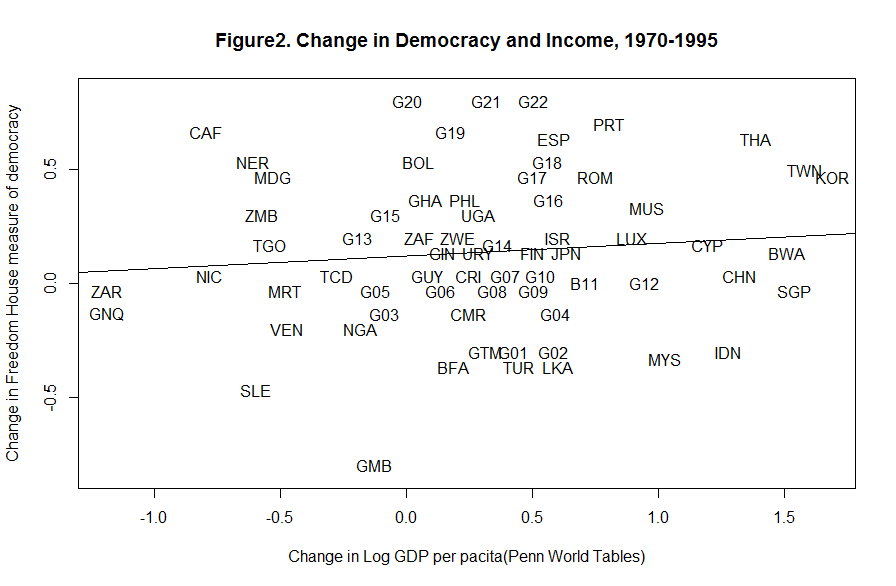
\includegraphics[width=15cm]{f2 fixed.png}
\end{center}
}
\begin{center}
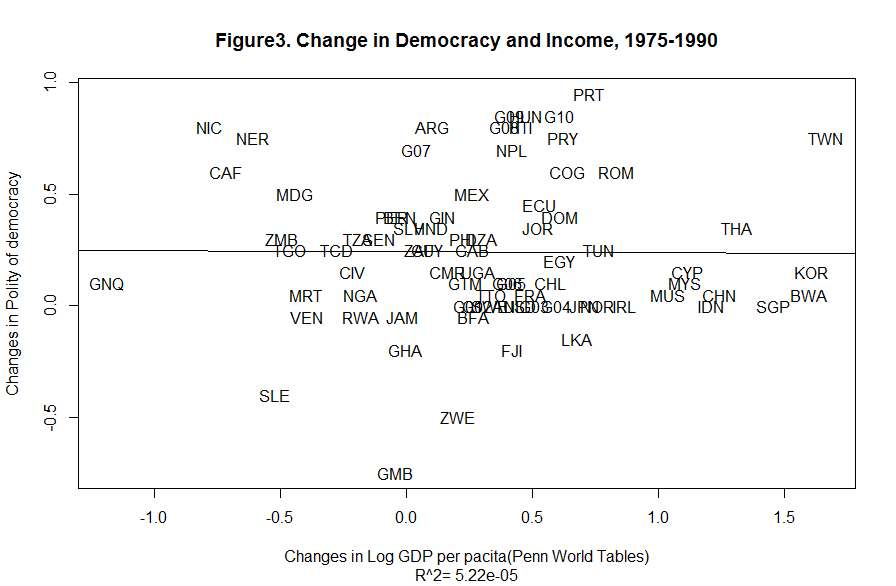
\includegraphics[width=15cm]{Figure3.png}
\end{center}
}


\begin{center}
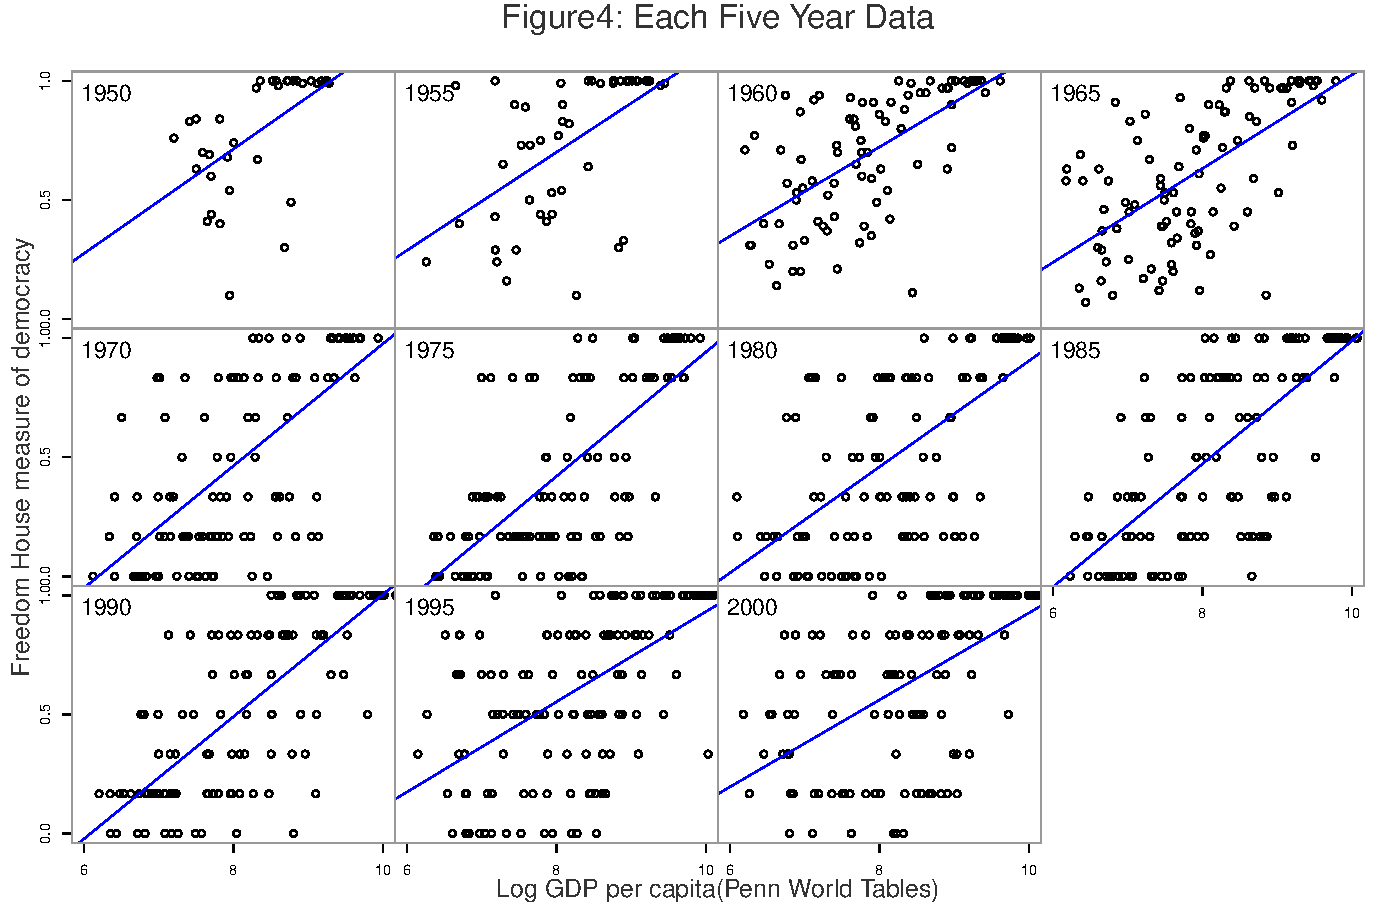
\includegraphics[width=15cm]{F4final.pdf}
\end{center}
}


\subsection{Regression Specification: Hyerin}
\ \ \ In this section, we discuss the causal effect of income on democracy. The relation between democracy scores and income per capita is estimated using the following simple econometric model:  
\begin{align}
d_{i,t} = \alpha d_{i,t-1} + \gamma y_{i,t-1}+ X'_{i,t-1}\beta + \mu_{t}+\delta_{i} + u_{i,t}
\end{align}
\ \ \ \ The democracy score of coutry $i$ in time period $t$ is denoted by $d_{i,t}$. To capture persistency of it, the lagged value of this variable, $d_{i,t}$, is included as a regressor in the model. $y_{i,t-1}$ denotes the lagged value of country $i$'s log income per capita and the estimated coefficient, $\gamma$, measures the causal effect of income per capita on democracy. If an increase in income per capita leads to an higher score of democracy, then the coefficient on the lagged value of log income per capita $\gamma$ should be positive. A full set of coutry dummies and time effects   $\delta_{i}$ $\mu_{t}$. All other potential covariates are denoted in the vector formation,  $X'_{i,t-1}$. To control for country-specific factors a full set of country dummies, $\delta_{i}$, is included in the right-hand side. In addition, to capture common shocks over all sample countries, it introduces $\mu_{t}$ as a full set of time effects. An error term is denoted as $u_{i,t}$.\\


\subsection{Regression Estimates}
\subsubsection{Fixed Effects: Soichi}
\\
Table 2 shows result of our estimation. We use 1960-2000 data of Freedom House Index as a proxy of democracy. All standard errors in the paper robust against heteroskedasticity and serial correlation at the country level.\\
First column in Table 2 shows result of our analysis with Standard Pooled OLS which is most typical way of estimate in the recent literature using the five-year data and dependent variable is five-year democracy data and independent variables are lagged five-year democracy and GDP per capita data. These lagged variables function as the country variables and full set of time series dummies. Though the result, lagged democracy and GDP per capita shows highly statistically significant. A coefficient of lagged democracy is 0.706, so we can say it has large effect, however, lagged GDP per capita is only 0.072 with 0.010 standard error. Therefore, in this estimation we can say that an impact of income per capita to democracy is too small and limited to take consider. \\
Other results in Table 2 show results through fixed effect. Colum 2 shows result of fixed effect OLS with same variables with the estimation of column 1. Democracy coefficient is 0.010 and since a standard error is 0.035, this coefficient is statistically insignificant. Thorough this estimation, we can say that the effect of logged GDP per capita disappears if we use fixed effect OLS.  \\
Column 3 shows a result of more simple model. In this model, we estimate a model of which independent variable is only lagged GDP per capita with fixed effect OLS by using five-year data. The result of this estimation shows that a coefficient of GDP per capita is only 0.054 and this is smaller than that of column 1, therefore it is too limited to take consider through this model. Moreover, in this case, the two standard error band comfortably exclude the corresponding OLS coefficient.\\
Also, we analyze the model with more longer lagged term data. Colum 4 shows the result of estimation of ten-year lagged and column 5 is twenty-year lagged. Because of lack of time series data, the number of twenty-year lagged data is smaller than others. Results of these estimations of effect of logged GDP per capita to democracy score are both statistically insignificant.\\
We can recognize these results by seeing figure2. Its vertical axis means change in the Freedom House Index and horizontal axis is change in GDP per capita for each country. It shows there is no significant relation between income and democracy same as our results.
\begin{table}[h!] \centering
			\begin{adjustbox}{max width=\textwidth}
			\begin{threeparttable}
		\caption{\textsc{fixed effects results using freedom house measure of democracy}}
			\begin{tabular}{l*{7}{c}} 
		 \hline\hline
			    & \multicolumn{7}{c}{Base sample, 1960-2000}\\
	     \cline{2-8}
	            & & &&& & &Twenty-year\\[-1.8ex]
				& \multicolumn{3}{c}{Five-year data} && \multicolumn{1}{c}{Ten-year data} && \multicolumn{1}{c}{data}\\
		\cline{2-4}\cline{6-6}\cline{8-8}	
		    &Pooled &Fixed effects &Fixed effects &&Fixed effects &&Fixed effects \\[-1.8ex] 	
		    &OLS &OLS &OLS &&OLS &&OLS \\[-1.8ex] 			 
		        &\multicolumn{1}{c}{(1)} &\multicolumn{1}{c}{(2)} &\multicolumn{1}{c}{(3)} &&\multicolumn{1}{c}{(4)} &&\multicolumn{1}{c}{(5)}\\ 
		\hline
		 & \multicolumn{7}{c}{\textit{Dependent variable is democracy}}\\        
			Democracy$_{t-1}$ & 0.706$^{***}$ & 0.379$^{***}$ &  && -0.025 && -0.581$^{***}$ \\[-1.8ex] 
				 \ & (0.035) & (0.051) &  && (0.088) && (0.198) \\ 
				Log GDP per capita${}_{t-1}$ & 0.072$^{***}$ & 0.010 & 0.054 && 0.053 && -0.030 \\[-1.8ex] 
				 \ & (0.010) & (0.035) & (0.046) && (0.066) && (0.156) \\ 
				Observations & \multicolumn{1}{c}{945} & \multicolumn{1}{c}{945} & \multicolumn{1}{c}{958} && \multicolumn{1}{c}{457} && \multicolumn{1}{c}{192} \\ 
				R${}^{2}$ & \multicolumn{1}{c}{0.725} & \multicolumn{1}{c}{0.242} & \multicolumn{1}{c}{0.118} && \multicolumn{1}{c}{0.122} && \multicolumn{1}{c}{0.452} \\ 
				\hline 
			\end{tabular}
		\begin{tablenotes}
					    	\item \textit{Notes:Column1 is pooled cross-sectional OLS regression with robust standard error clustered by country in parentheses. Column2 to 5 are fixed effect OLS with country dummies and robust standard errors clustered by country in parentheses. Year dummies are included in all regressions. Dependent variable is Freedom House measure of democracy. First year of dependent variable data in all columns are 1960, and year of independent variables begin with subtract year of interval from 1960. For example, in column 1, first year data of dependent variable is 1960 and independent variable is 1955 since interval is 5 year. All the countries in sample data exist during interval term. For example, in column5, all counties analyzed in independent variable of 1960 data, country should exist before 1940.} 
		\end{tablenotes}
		\end{threeparttable}	
		\end{adjustbox}
	\end{table}

\begin{itemize}
    \item Organize material and present results.
    \item Use tables, figures (but prefer visual presentation):
        \begin{itemize}
            \item Tables and figures should supplement (and not duplicate) the text.
            \item Tables and figures should be provided with legends.\\
                {\it Figure \ref{Fig:Resids} shows how to include and reference
                graphics. The graphic must be labelled before. Files must be in
                \texttt{.eps} format.}

                \begin{figure}[ht]
                \begin{center}
                    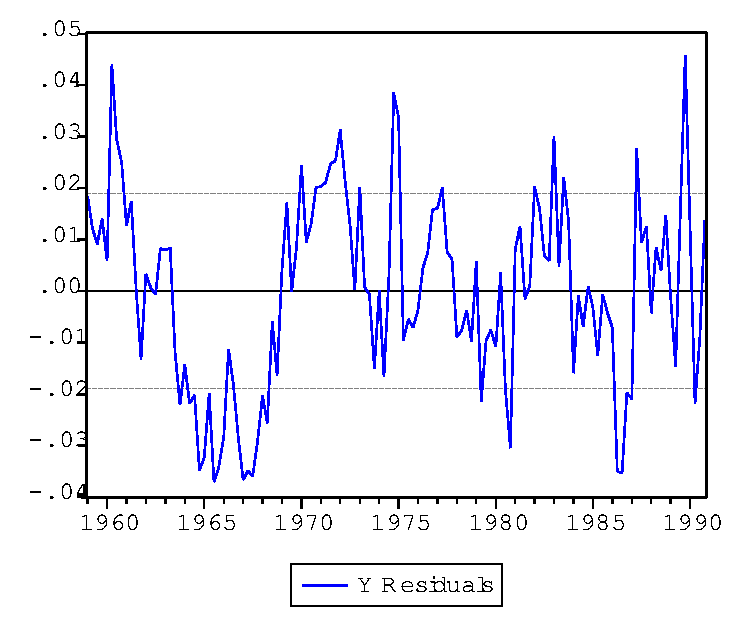
\includegraphics[scale=0.5,angle=0]{graph}
                    \caption{Estimated residuals from model XXX. ...}
                    \label{Fig:Resids}
                \end{center}
                \end{figure}

            \item Tables and graphics may appear in the text or in the appendix, especially if there are many simulation result tabulated, but is also depends on the study and number of tables resp.figures. The key graphs and tables must appear in the text!
        \end{itemize}
 \end{itemize}   
\subsubsection{Instrumental Variable: Hyerin}
Since the fixed effects estimation does not necessarily examine the causal effect of income on democracy, we need a instrumental variable to estimate the causal relation betweem them.    
	\begin{table}[h!] 
		\centering
		\begin{adjustbox}{max width=\textwidth}
		\begin{threeparttable}
			\caption{\textsc{fixed effects results using freedom house measure of democracy: Two-stage least squares with savings rate instrument}}			
			\begin{tabular}{lcccccccc}
		    \hline\hline
		    \ &\multicolumn{8}{c}{Base sample, 1960-2000}\\
		    \cline{2-9}
		    \ &\multicolumn{8}{c}{All countries}\\
		    \cline{2-9}
		    &Pooled &Fixed effects &Fixed effects &Fixed effects &Fixed effects &Fixed effects &Fixed effects &Fixed effects\\[-1.8ex] 	
		    &OLS &OLS &OLS &2SLS &2SLS &2SLS &2SLS &2SLS\\[-1.8ex] 
		    &(1) &(2) &(3) &(4) &(5) &(6) &(7) &(8)\\
		    \hline 
			Panel A &\multicolumn{8}{c}{\textit{Dependent variable is democracy}}\\			
			\hline
			Democracy${}_{t-1}$ &  &  & 0.359 &  & 0.363 &  &  &\\[-1.8ex] 
				&  &  &(0.054) &  & (0.056) &  &  &  \\ 
			Log GDP per capita${}_{t-1}$ & 0.233$^{***}$ & 0.044 & 0.009 & -0.035 & -0.020 & -0.036 & -0.074 & 0.016 \\[-1.8ex] 
				& (0.013) & (0.051) & (0.038) & (0.094) & (0.081) & (0.191) & (0.113) & (0.095) \\ 
			Labor share${}_{t-1}$ &  &  &  &  &  & 0.250 &  &  \\[-1.8ex] 
				&  &  &  &  &  & (0.199) &  &  \\
			\hline
			Panel B &\multicolumn{8}{c}{\textit{First stage for log GDP per capita$_{t-1}$}}\\
			\hline			
			Democracy${}_{t-1}$ &  &  &  &  & 0.144$^{**}$ &  & [0.24] &  \\[-1.8ex] 
				&  &  &  &  & (0.066) &  &  &  \\ 
			Labor share${}_{t-1}$ &  &  &  &  &  & 0.329$^{*}$ &  &  \\[-1.8ex] 
				&  &  &  &  &  & (0.187) &  &  \\ 
			Savings rate${}_{t-2}$ &  &  &  & 1.356$^{***}$ & 1.343$^{***}$ & 1.202$^{***}$ & 1.173$^{***}$ & 1.022$^{***}$ \\[-1.8ex] 
				&  &  &  & (0.277) & (0.270) & (0.315) & (0.254) & (0.218) \\ 
			Savings rate${}_{t-3}$ &  &  &  &  &  &  &  & 0.720$^{***}$ \\[-1.8ex] 
				&  &  &  &  &  &  &  & (0.182) \\ 
				Observations &\multicolumn{1}{c}{891} & \multicolumn{1}{c}{900} & \multicolumn{1}{c}{766} & \multicolumn{1}{c}{900} & \multicolumn{1}{c}{891} & \multicolumn{1}{c}{471} & \multicolumn{1}{c}{733} & \multicolumn{1}{c}{796} \\ 
				R$^{2}$ &\multicolumn{1}{c}{0.226} & \multicolumn{1}{c}{0.115} & \multicolumn{1}{c}{0.225} & \multicolumn{1}{c}{0.571} & \multicolumn{1}{c}{0.571} & \multicolumn{1}{c}{0.725} & \multicolumn{1}{c}{0.541} & \multicolumn{1}{c}{0.536} \\ 
				\hline
			\end{tabular}
		    \begin{tablenotes}
		    	\item \textit{Notes:} This table summarizes the codefficients of each cross-sectional regression. All regression model includes year dummies to capture country-invariant factors. Except for column 1, country dummies are included in the regressions. The robust standrad errors clustered by country are summarized in parentheses. 
		    	\item \begin{align}
		    	^{***}& \text{Significant at the 1 percent level}\notag\\
		    	^{**}& \text{Significant at the 5 percent level}\notag\\
		    	^{*}& \text{Significant at the 10 percent level}\notag
		    	\end{align}
		    \end{tablenotes}
		\end{threeparttable}
		\end{adjustbox}			
	\end{table} 	


\newpage
\subsection{Robustness Tests: Sharon}
\begin{table}[h!] \centering
	\begin{adjustbox}{max width=\textwidth}
		\begin{threeparttable}
			\caption{\textsc{Fixed effects results with alternative samples and additional control variables}}			
			\begin{tabular}{l*{6}{c}} 
			\hline\hline
			& \multicolumn{6}{c}{Five-year data}\\
            \cline{2-7}
			&Balanced panel &&Base sample, 1960-2000, &&&\\[-1.8ex] 
			&1970-2000 &&without former socialist countries  & &\multicolumn{2}{c}{Base sample, 1960-2000}\\
			\cline{2-2} \cline{4-4} \cline{6-7} 
			&Fixed effects &&Fixed effects &&Fixed effects &Fixed effects \\[-1.8ex] 	
			&OLS &&OLS &&OLS&OLS \\[-1.8ex] 			 
&\multicolumn{1}{c}{(1)} &&\multicolumn{1}{c}{(2)} &&\multicolumn{1}{c}{(3)}&\multicolumn{1}{c}{(4)} \\ 
\hline				
&\multicolumn{6}{c}{\textit{Dependent variable is democracy}}\\	
\cline{2-7}	
Democracy$_{t-1}$ & 0.283$^{***}$ && 0.362$^{***}$ && 0.353$^{***}$ & 0.351$^{***}$ \\ [-1.8ex]
& (0.058) && (0.052) && (0.053) & (0.055) \\ 
Log GDP per capita$_{t-1}$ & -0.031 && 0.005 && 0.015 & -0.001 \\ 
& (0.049) && (0.035) && (0.041) & (0.049) \\[-1.8ex] 
Log population$_{t-1}$ &  &&  && -0.109 & -0.042 \\ 
&  &&  && (0.100) & (0.108) \\ 
Education$_{t-1}$ &  &&  &&  & -0.007 \\ [-1.8ex]
&  &&  &&  & (0.020) \\ 
Age Structure$_{t-1}$ &  &&  && [0.05] & [0.19] \\
Observations & \multicolumn{1}{c}{630} && \multicolumn{1}{c}{908} && \multicolumn{1}{c}{863} & \multicolumn{1}{c}{676} \\[-1.8ex]
Countries &90 &&128 &&142 &95\\[-1.8ex] 
R$^{2}$ & \multicolumn{1}{c}{0.215} && \multicolumn{1}{c}{0.221} && \multicolumn{1}{c}{0.241} & \multicolumn{1}{c}{0.235} \\ 
\hline
\end{tabular}
\begin{tablenotes}
	\item \textit{Notes:} 
\end{tablenotes}
\end{threeparttable}	
\end{adjustbox}
\end{table}

\begin{table}[h] \centering
	\begin{adjustbox}{max width=\textwidth}
		\begin{threeparttable}
			\caption{\textsc{fixed effects results using an alternative dependent variable: polity measure}}			
			\begin{tabular}{l*{7}{c}} 
				\hline\hline
				& \multicolumn{7}{c}{Base sample, 1960-2000}\\
				\cline{2-8}
				& & &&& & &Twenty-year\\[-1.8ex]
				& \multicolumn{3}{c}{Five-year data} && \multicolumn{1}{c}{Ten-year data} && \multicolumn{1}{c}{data}\\
				\cline{2-4}\cline{6-6}\cline{8-8}	
				&Pooled &Fixed effects &Fixed effects &&Fixed effects &&Fixed effects \\[-1.8ex] 	
				&OLS &OLS &OLS &&OLS &&OLS \\[-1.8ex] 			 
				&\multicolumn{1}{c}{(1)} &\multicolumn{1}{c}{(2)} &\multicolumn{1}{c}{(3)} &&\multicolumn{1}{c}{(4)} &&\multicolumn{1}{c}{(5)}\\ 
				\hline 
				Democracy${}_{t-1}$ & 0.749$^{***}$ & 0.449$^{***}$ &  && 0.060 && -0.516$^{***}$ \\[-1.8ex]
				& (0.034) & (0.063) &  && (0.091) && (0.165) \\ 
				Log GDP per capita${}_{t-1}$ & 0.053$^{***}$ & -0.006 & -0.011 && 0.007 && -0.126 \\[-1.8ex] 
				& (0.010) & (0.039) & (0.055) && (0.070) && (0.164) \\ 
				Observations & \multicolumn{1}{c}{854} & \multicolumn{1}{c}{854} & \multicolumn{1}{c}{880} && \multicolumn{1}{c}{419} && \multicolumn{1}{c}{168} \\ 
				R$^{2}$ & \multicolumn{1}{c}{0.772} & \multicolumn{1}{c}{0.396} & \multicolumn{1}{c}{0.248} && \multicolumn{1}{c}{0.257} && \multicolumn{1}{c}{0.544} \\
				\hline 
			\end{tabular}
			\begin{tablenotes}
				\item \textit{Notes:} 
			\end{tablenotes}
		\end{threeparttable}	
	\end{adjustbox}
\end{table}
\begin{itemize}
    \item Discuss results:
        \begin{itemize}
            \item Do the results support or do they contradict economic theory ?
            \item What does the reader learn from the results?
            \item Try to give an intuition for your results.
            \item Provide robustness checks.
            \item Compare to previous research.
        \end{itemize}
\end{itemize}

\newpage
\section{Conclusions}\label{Sec:Conclusion}

\begin{itemize}

For long years, many researches and paper have suggested that democratic political system is inevitable for economic growth. However, these days, countries which do not have democratic political regime like China and Singapore, receive attention for large economic development. Therefore, we analyze to research weather there is a relation between democracy and income. We use Freedom House Political Right Index and PolityI\hspace{-.1em}V as proxies of democracy and GDP log per capita as an income proxies. We research by using fixed effect model and two-stage least square model and we expected that there is a positive relation between them. However, contrary to our expectation, there is no significant relationship between them in our econometric model, so we could not find significant relation between income and democracy. 

We analyze only post war era because data sets for Freedom House Political Right Index and PolityI\hspace{-.1em}V do not reliable and have enough data before the World War Second. But it might be causal significant relation if we research more long time series data. Also, in many articles suggest that democracy is necessary for economic growth, but there might exist a reverse causal relationship between income and democracy, for instance, income is crucial for democratic political systems.


\end{itemize}




% ----------------
% --- appendix ---
% ----------------
\appendix
\begin{center}
\includegraphics[width=15cm]{f1 fixed.png}
\end{center}
}
\begin{center}
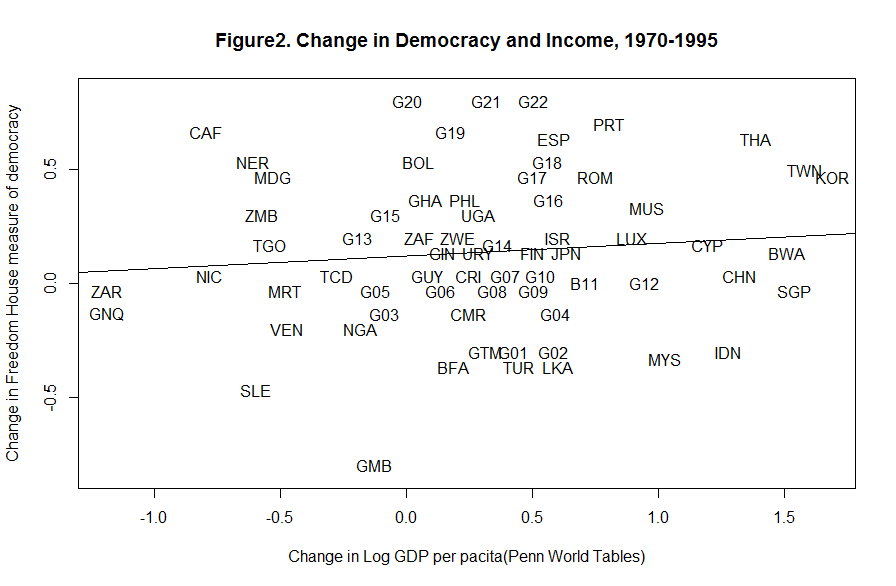
\includegraphics[width=15cm]{f2 fixed.png}
\end{center}
}
\begin{center}
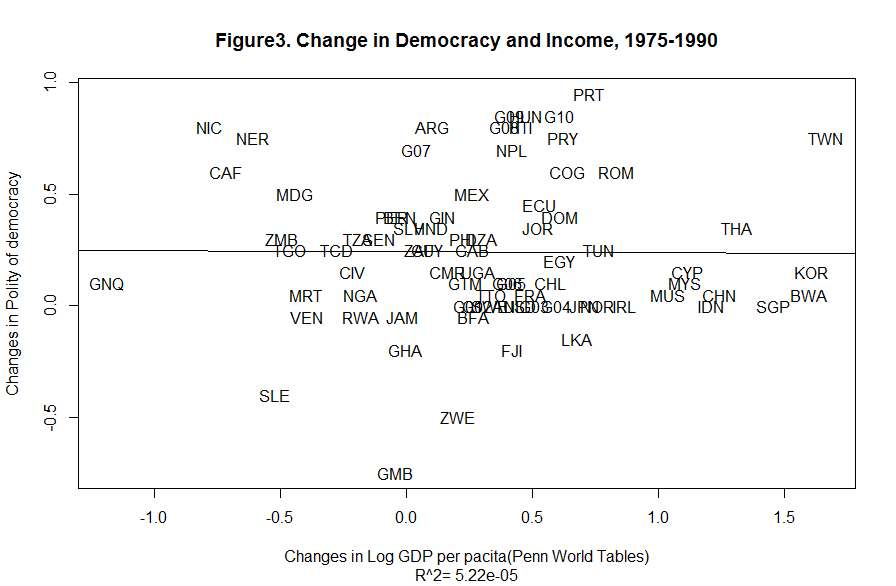
\includegraphics[width=15cm]{Figure3.png}
\end{center}
}


\begin{center}
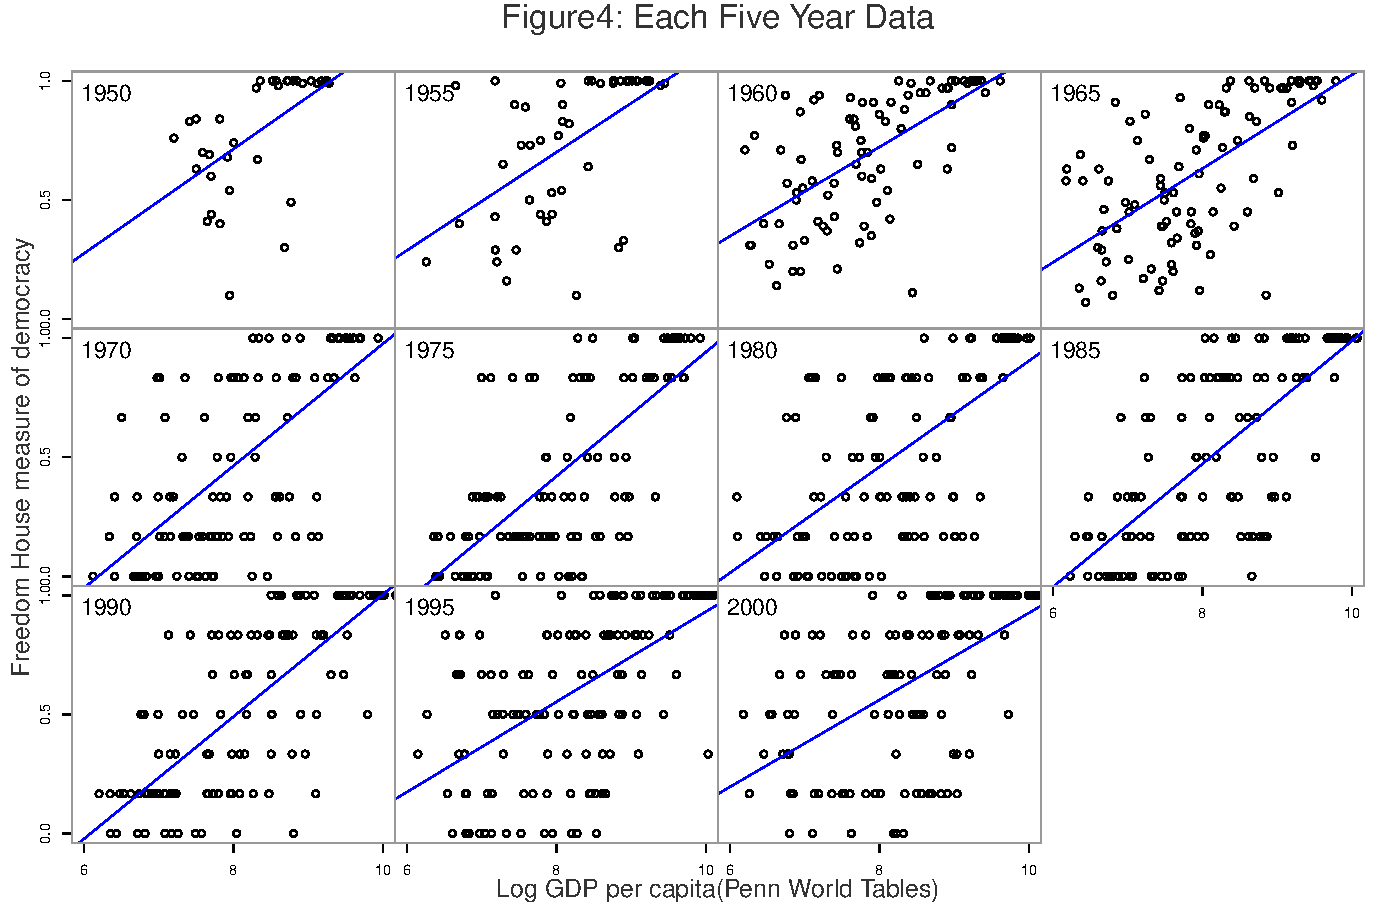
\includegraphics[width=15cm]{F4final.pdf}
\end{center}
}

% literature
\newpage
\addcontentsline{toc}{section}{References}
\bibliography{literature}
Heston, Alan, Robert Summer, and Bettina Aten 2002. Penn World Table Version6.1. Philadelphia: Center for International Comparisons at the University of Pennsylvania\\
http://datacentre2.chass.utoronto.ca/pwt61/\\
Barro, Robert J. 1999. "Determinants of Democracy." Journal of Political Economy, 107(6): S158–83\\
Bollen, Kenneth A. 1990. "Political Democracy: Conceptual and Measurement Traps." Studies in Comparative International development, 25(1): 7–24.\\
Bollen, Kenneth A. "Cross-National Indicators of Liberal Democracy, 1950–1990." and ICPSR version. Chapel Hill, NC: University of North Carolina, 1998. Inter-university Consortium for Political and Social Research, 2001.\\


% code
\newpage
\section{Source Code Listing}
\lstinputlisting[language=R]{./code/clustered_SEs.R}
\lstinputlisting[language=R]{./code/T2_wtests.R}
\lstinputlisting[language=R]{./code/T3_wtests.R}
\lstinputlisting[language=R]{./code/T4_wtests.R}
F1
\begin{lstlisting}
library(maptools)

result<-lm(fhpolrigaug~lrgdpch,data=F1_revise)
R2=signif(summary(result)$r.squared,digit=4)
R="R^2="

plot(fhpolrigaug~lrgdpch,data=F1_revise,col="white",
ylab="Freedom House measure of democracy",xlab="Log GDP per pacita(Penn World Tables)",
main="Figure1.Democacy and Income , 1990s",sub=paste(R,R2))
pointLabel(x=F1_revise$lrgdpch,y=F1_revise$fhpolrigaug,labels=F1_revise$code,col="black")

abline(result)

\end{lstlisting}

\\
F2
\begin{lstlisting}
library(maptools)

result<-lm(s5fhpolrigaug~s5lrgdpch,data=F2)
R2=signif(summary(result)$r.squared,digit=4)
R="R^2="

plot(s5fhpolrigaug~s5lrgdpch,data=F2,type="n",
ylab="Change in Freedom House measure of democracy",xlab="Change in Log GDP per pacita(Penn World Tables)",
main="Figure2. Change in Democracy and Income, 1970-1995")
pointLabel(x=F2$s5lrgdpch,y=F2$s5fhpolrigaug,labels=F2$code)
resultf2<-lm(s5fhpolrigaug~s5lrgdpch,data=F2)
abline(resultf2)


\end{lstlisting}

\\
F3
\begin{lstlisting}
library(maptools)

result3<-lm(s5polity4~s5lrgdpch,data=F3)
R2.3=signif(summary(result3)$r.squared,digit=4)
R="R^2="

plot(s5polity4~s5lrgdpch,data=F3,type="n",
ylab="Changes in Polity of democracy",xlab="Changes in Log GDP per pacita(Penn World Tables)",
main="Figure3. Change in Democracy and Income, 1975-1990",sub=paste(R,R2.3))
pointLabel(x=F3$s5lrgdpch,y=F3$s5polity4,labels=F3$code)

abline(result3)


\end{lstlisting}

\\
F4
\begin{lstlisting}
par(mfrow = c(3,4 ))          ##par is graphic parameter, mflow is to devide the graph in 12 areas
par(cex = 0.6)                #zoom rate for characters
par(mar = c(0, 0, 0, 0), oma = c(4, 4, 4, 2))  #oma is for setting vacant space

x<-1945
for (i in 1:11) {
x<-x+5
plot(fhpolrigaug~lrgdpch,data=X5yr_panel, subset=year==x,
xlim=c(6,10),ylim=c(0,1),ann=F, xaxt="n",yaxt="n")  #setting for length of graph by xlim and ylim, and erase whole title and axis by ann=F
text(6.3,0.95,x, cex=1.5)     #label setting for each graph
if (i %in% c (8:11) ) { axis (1 , col = " black ", col.axis= " black ", at = seq (6 , 10 , 2) ) }
if (i %in% c(1 , 5 , 9) ) { axis (2 , col = " black ", col.axis = " black ", at = seq (0 , 1 , 0.5) ) }
result<-lm(formula=fhpolrigaug~lrgdpch, data=X5yr_panel, subset=year==x)
abline(result, col="blue")
box(col = "grey60")
mtext("Freedom House measure of democracy", 
side = 2, outer = TRUE, cex = 1, line = 2.2,col = "grey20")
mtext("Log GDP per capita(Penn World Tables)", 
side = 1, outer = TRUE, cex = 1, line = 2.2,col = "grey20")
mtext("Figure4: Each Five Year Data", 
side = 3, outer = TRUE, cex = 1.3, line = 2.2,col = "grey20")

\end{lstlisting}

F1
\begin{lstlisting}
library(maptools)

result<-lm(fhpolrigaug~lrgdpch,data=F1_revise)
R2=signif(summary(result)$r.squared,digit=4)
R="R^2="

plot(fhpolrigaug~lrgdpch,data=F1_revise,col="white",
     ylab="Freedom House measure of democracy",xlab="Log GDP per pacita(Penn World Tables)",
     main="Figure1.Democacy and Income , 1990s",sub=paste(R,R2))
pointLabel(x=F1_revise$lrgdpch,y=F1_revise$fhpolrigaug,labels=F1_revise$code,col="black")

abline(result)

\end{lstlisting}

\\
F2
\begin{lstlisting}
library(maptools)

result<-lm(s5fhpolrigaug~s5lrgdpch,data=F2)
R2=signif(summary(result)$r.squared,digit=4)
R="R^2="

plot(s5fhpolrigaug~s5lrgdpch,data=F2,type="n",
     ylab="Change in Freedom House measure of democracy",xlab="Change in Log GDP per pacita(Penn World Tables)",
     main="Figure2. Change in Democracy and Income, 1970-1995")
pointLabel(x=F2$s5lrgdpch,y=F2$s5fhpolrigaug,labels=F2$code)
resultf2<-lm(s5fhpolrigaug~s5lrgdpch,data=F2)
abline(resultf2)


\end{lstlisting}

\\
F3
\begin{lstlisting}
library(maptools)

result3<-lm(s5polity4~s5lrgdpch,data=F3)
R2.3=signif(summary(result3)$r.squared,digit=4)
R="R^2="

plot(s5polity4~s5lrgdpch,data=F3,type="n",
     ylab="Changes in Polity of democracy",xlab="Changes in Log GDP per pacita(Penn World Tables)",
     main="Figure3. Change in Democracy and Income, 1975-1990",sub=paste(R,R2.3))
pointLabel(x=F3$s5lrgdpch,y=F3$s5polity4,labels=F3$code)

abline(result3)


\end{lstlisting}

\\
F4
\begin{lstlisting}
par(mfrow = c(3,4 ))          ##par is graphic parameter, mflow is to devide the graph in 12 areas
par(cex = 0.6)                #zoom rate for characters
par(mar = c(0, 0, 0, 0), oma = c(4, 4, 4, 2))  #oma is for setting vacant space

x<-1945
for (i in 1:11) {
  x<-x+5
  plot(fhpolrigaug~lrgdpch,data=X5yr_panel, subset=year==x,
       xlim=c(6,10),ylim=c(0,1),ann=F, xaxt="n",yaxt="n")  #setting for length of graph by xlim and ylim, and erase whole title and axis by ann=F
  text(6.3,0.95,x, cex=1.5)     #label setting for each graph
  if (i %in% c (8:11) ) { axis (1 , col = " black ", col.axis= " black ", at = seq (6 , 10 , 2) ) }
  if (i %in% c(1 , 5 , 9) ) { axis (2 , col = " black ", col.axis = " black ", at = seq (0 , 1 , 0.5) ) }
  result<-lm(formula=fhpolrigaug~lrgdpch, data=X5yr_panel, subset=year==x)
  abline(result, col="blue")
  box(col = "grey60")
}
mtext("Freedom House measure of democracy", 
      side = 2, outer = TRUE, cex = 1, line = 2.2,col = "grey20")
mtext("Log GDP per capita(Penn World Tables)", 
      side = 1, outer = TRUE, cex = 1, line = 2.2,col = "grey20")
mtext("Figure4: Each Five Year Data", 
      side = 3, outer = TRUE, cex = 1.3, line = 2.2,col = "grey20")

\end{lstlisting}

% figures (not mandatory)
\newpage
\section{Figures}

\begin{figure}[ht]
    \begin{center}
        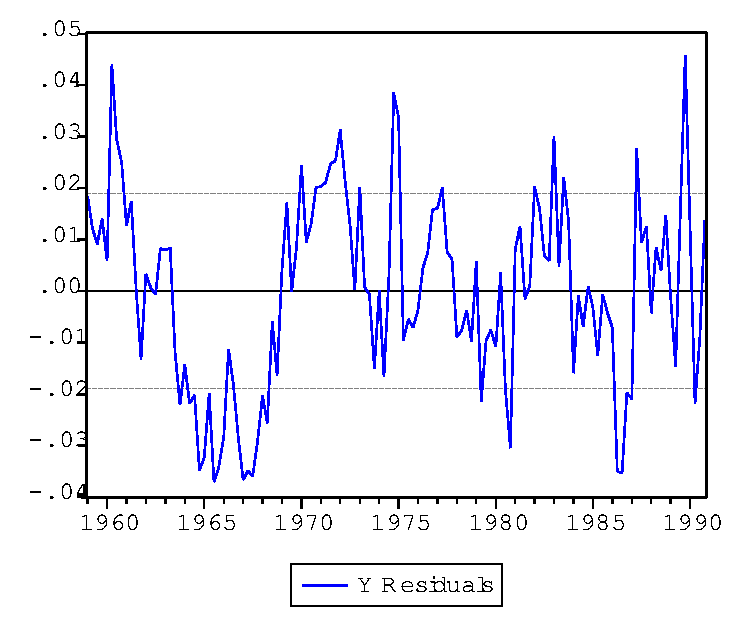
\includegraphics[scale=0.5,angle=0]{graph}
        \caption{Estimated residuals (2) from model XXX. ...}
        \label{Fig:Resids2}
    \end{center}
\begin{center}
	\includegraphics[width=15cm]{f1 notitle.pdf}
	\caption{Figure1: Democracy And Income}
\end{center}
}
\begin{center}
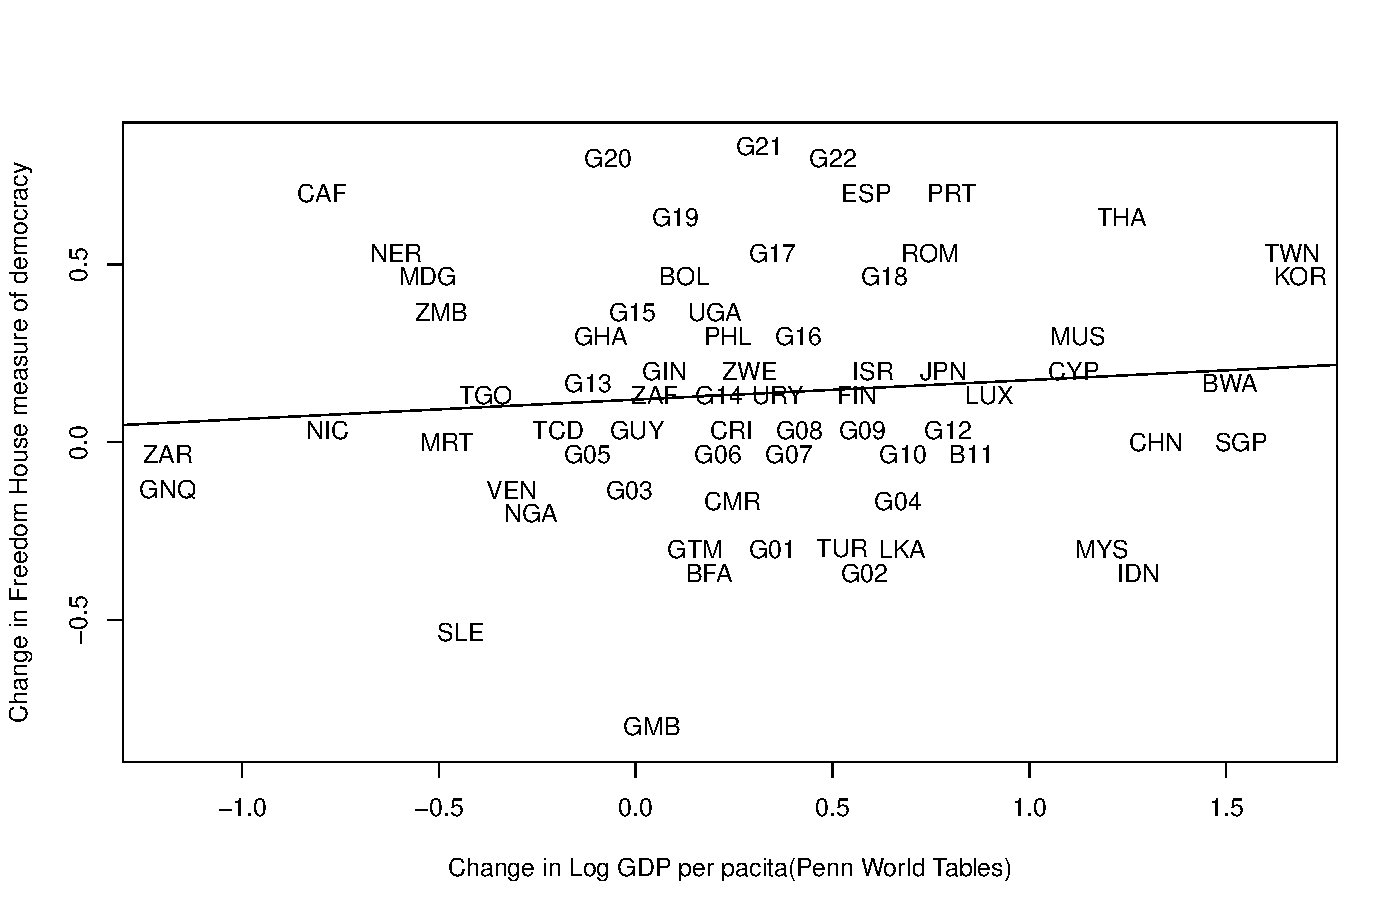
\includegraphics[width=15cm]{f2notitle.pdf}
\caption{Figure2: Change In Democracy And Income, 1970-1995}
\end{center}
}
\begin{center}
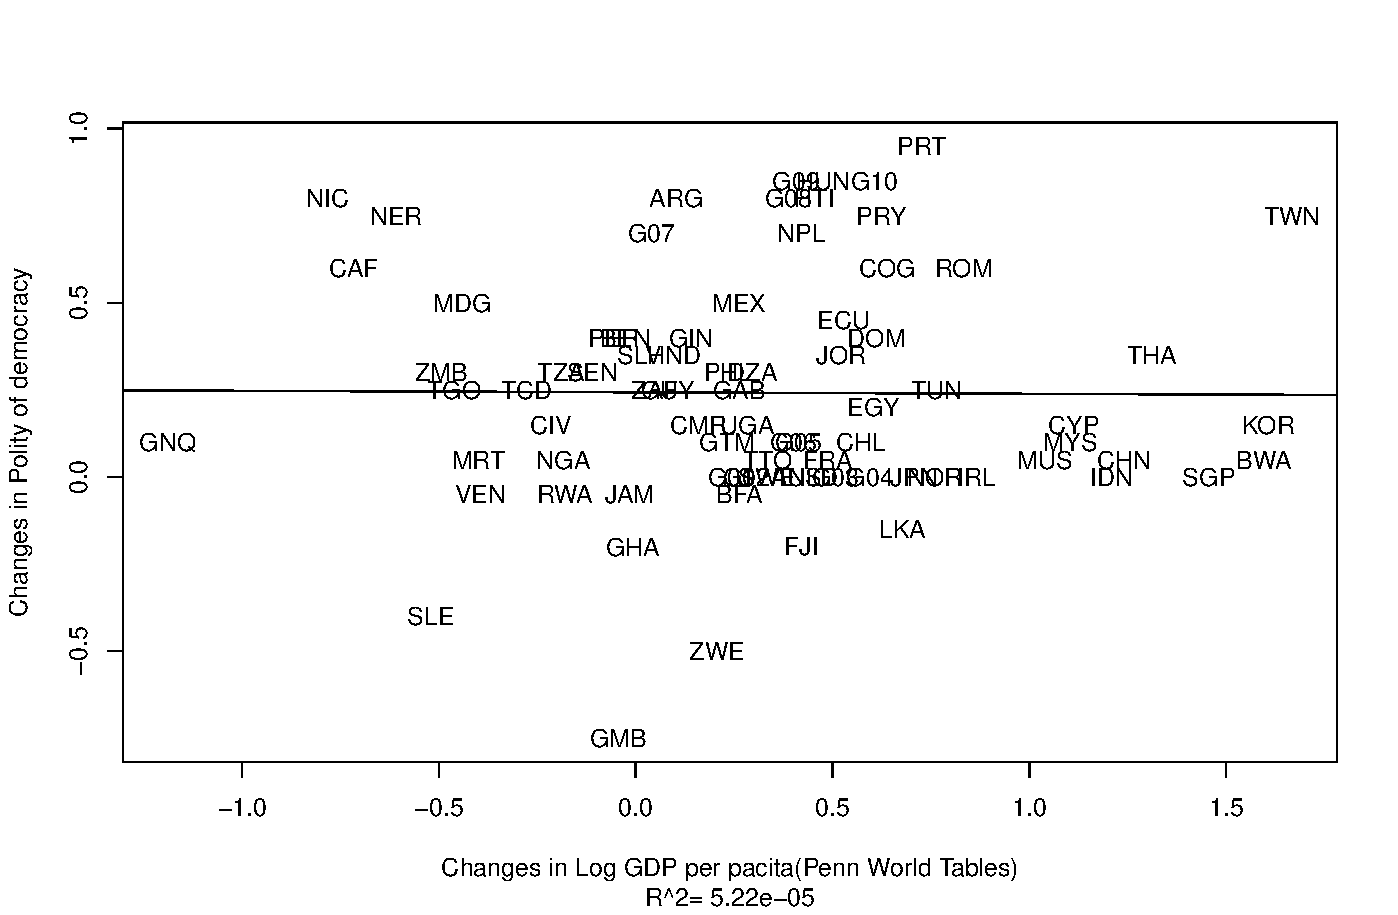
\includegraphics[width=15cm]{f3nofile.pdf}
\caption{Figure3: Change In Democracy And Income, 1970-1995}
\end{center}
}


\begin{center}
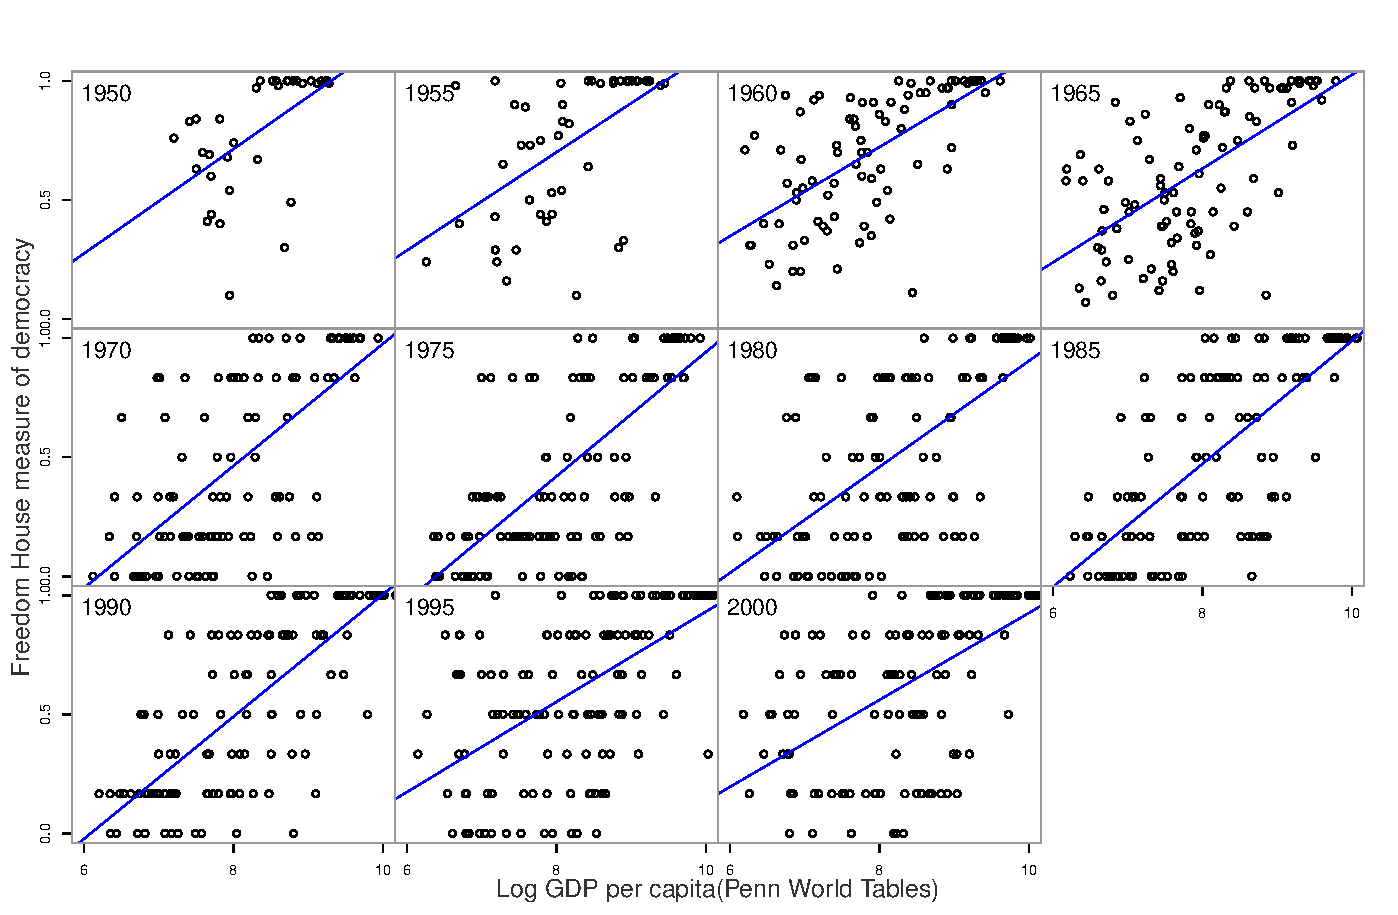
\includegraphics[width=15cm]{f4notitle.pdf}
\caption{Figure4: Five-Year Panel Data}
\end{center}
}

\end{figure}


% tables (not mandatory)
\newpage
\section{Tables}

\begin{table}[ht]
    \begin{center}
        {\footnotesize
        \begin{tabular}{l|cccccccccc}
        \hline \hline
                        & 3m    & 6m    & 1yr   & 2yr   & 3yr   & 5yr   & 7yr   & 10yr  & 12yr  & 15yr   \\
            \hline
                Mean   & 3.138 & 3.191 & 3.307 & 3.544 & 3.756 & 4.093 & 4.354 & 4.621 & 4.741 & 4.878  \\
                Median & 3.013 & 3.109 & 3.228 & 3.490 & 3.680 & 3.906 & 4.117 & 4.420 & 4.575 & 4.759  \\
                Min    & 1.984 & 1.950 & 1.956 & 2.010 & 2.240 & 2.615 & 2.850 & 3.120 & 3.250 & 3.395  \\
                Max    & 5.211 & 5.274 & 5.415 & 5.583 & 5.698 & 5.805 & 5.900 & 6.031 & 6.150 & 6.295  \\
                StD    & 0.915 & 0.919 & 0.935 & 0.910 & 0.876 & 0.825 & 0.803 & 0.776 & 0.768 & 0.762  \\
            \hline \hline
        \end{tabular}}
    \end{center}
    \caption{Detailed descriptive statistics of location and dispersion for
    2100 observed swap rates for the period from
    February 15, 1999 to March 2, 2007. Swap rates measured as 3.12 (instead of 0.0312).}
    \label{Tab:DescripStatsRawDataDetail}
\end{table}




% --------------------------------------------
% --- last page: Declaration of Authorship ---
% --------------------------------------------

%\newpage
%\thispagestyle{empty}
%%{\Large{\bf Declaration of Authorship}}\vspace{0.5cm}

\section*{Declaration of Authorship}

I hereby confirm that I have authored this Bachelor's/Master's
thesis independently and without use of others than the indicated
sources. All passages which are literally or in general matter
taken out of publications or other sources are marked as such.
\vspace{1cm}

Berlin, September 30, 2007 \vspace{0.5cm}

your name (and signature, of course)



\end{document}
